% Keep these two lines in order to get typesetting to work w/ the funny fonts.
%!TEX TS-program = xelatex
%!TEX encoding = UTF-8 Unicode

\documentclass[12pt]{article}
\usepackage{geometry} % See geometry.pdf for lots of layout options. 
\usepackage{graphicx}
\usepackage{amssymb}
\usepackage[small,compact]{titlesec}
\usepackage[small,it]{caption}

\usepackage{fontspec,xltxtra,xunicode}
\defaultfontfeatures{Mapping=tex-text}
\setromanfont[Mapping=tex-text]{Times New Roman}
\setsansfont[Scale=MatchLowercase,Mapping=tex-text]{Gill Sans}
\setmonofont[Scale=MatchLowercase]{Andale Mono}

\newenvironment{packed_enum}{
\begin{enumerate}
  \setlength{\itemsep}{1pt}
  \setlength{\parskip}{0pt}
  \setlength{\parsep}{0pt}
}{\end{enumerate}}

\newcommand{\squishlist}{
 \begin{list}{$\rightarrow$} % cdot or bullet or circ or rightarrow
  { \setlength{\itemsep}{0pt}
     \setlength{\parsep}{3pt}
     \setlength{\topsep}{3pt}
     \setlength{\partopsep}{0pt}
     \setlength{\leftmargin}{1.5em}
     \setlength{\labelwidth}{1em}
     \setlength{\labelsep}{0.5em} } }

\newcommand{\squishlisttwo}{
 \begin{list}{$\bullet$}
  { \setlength{\itemsep}{0pt}
     \setlength{\parsep}{0pt}
    \setlength{\topsep}{0pt}
    \setlength{\partopsep}{0pt}
    \setlength{\leftmargin}{2em}
    \setlength{\labelwidth}{1.5em}
    \setlength{\labelsep}{0.5em} } }

\newcommand{\squishend}{
  \end{list}  }

\title{Thoughts and Such}
\author{Gabe Johnson}
\date{July 11 (or so) 2011} % Activate to display a given date or no date

\begin{document}
\maketitle

% \begin{abstract}
% Put your abstract here and uncomment.
% \end{abstract}


\section{Fluidity}
\textit{Fluidity} is often cited as one of the properties of
pencil-and-paper sketching that makes it such a powerful practice. We
say that it is fluid because users may:

\begin{packed_enum}
\item draw on any suitable location at any time...
\item branch off to new or different ideas at any time...
\item delve into details of particular ideas...
\item simultaneously see earlier drawings...
\item re-draw complete or partial drawings...
\end{packed_enum}

Perhaps the benefit of paper sketching is not simply that users enjoy
all of the above abilities, but that it \textit{doesn't} have
detrimental properties commonly associated with computer
tools. Typical computer design software:

\begin{packed_enum}
\item demands that users provide information that (to the user) is not
  yet known or relevant
\item has modes that restrict what users may do at any given time or
  location
\item guides designers to think and work in terms of the tool's
  worldview
\end{packed_enum}

\begin{table}[t] %
\centering
\begin{tabular}{|r|p{7.0cm}|p{7.0cm}|}
\hline
 & Paper \& Pencil & Computer \\
\hline
Good &
\squishlist
\item draw wherever
\item no modes
\item change to new or different idea at leisure
\item give only details when known or needed
\item see other ideas or sketches on page
\item redraw/erase as desired
\item be as abstract or detailed as needed
\squishend
&
\squishlist
\item interact with typed or recognized objects
\item can specify parameters and values
\item modes enable unambiguous actions
\item gives computed feedback (e.g. critics and compilers)
\item can run, simulate, print, or manufacture models
\item good for distributed collaboration
\item not physically unique
\squishend
\\
\hline
Bad &
\squishlist
\item meaning entirely in mind of viewer
\item physically unique (can be lost/destroyed), must have access to see it
\item takes skill to make good, accurate sketches
\item difficult to search large collections of sketches
\squishend
&
\squishlist
\item demands information of designer prematurely
\item modes restrict actions and impose cognitive load
\item forces users to think in terms of tool's worldview
\squishend
\\
\hline
\end{tabular}
\caption{Helpful and hindering properties of paper sketching compared
  with standard computer design tools.}
\label{tab:helpful-hinder}
\end{table}

Table \ref{tab:helpful-hinder} is a 2x2 matrix of the positive and
negative aspects of paper sketching and computer design software. It
would be a victory for designer-centered computer sketching tools to
retain the good properties while removing or mitigating the bad ones.
The unwanted aspects of each activity are those that break flow. I
won't directly address all of them---e.g. I will not be developing a
psychic machine with respect to the meaning of sketches ``entirely in
mind of viewer''. Some other aspects (uniqueness of physical sketches)
are addressed easily. In the middle are interesting interaction
challenges: making it easier to sketch with a computer while also
being able to specify via sketching.

My thesis proposal declared that I would build ``a coherent set of
calligraphic interaction techniques for iteratively making structured
drawings that have enough detail that objects can be fabricated on a
laser cutter''. This thesis is about \textit{iterative, conversational
  sketch-based interaction}.

\textit{Iterative}: Designers arrive at their final products after a
series of starts and stops. Along the way, high-level ideas are
considered, drawings are made, specifications are given. This does not
happen linearly. An idea may be abandoned temporarily as another is
recorded and explored, only to be (potentially) resumed later on. Even
aborted ideas have value as examples of what is \textit{not}
wanted.

\textit{Conversational}: The proposed system knows something about the
domain and the kind of drawings people are likely to make. When
appropriate, it will be an active participant in the design process by
re-structuring and cleaning up drawings, asking questions about
ambiguous parts, and providing contextually-derived help.

\textit{Sketch-based interaction}: The tool will be based on freehand
pen input. This will largely be recognized without needing to be in
specific drawing modes (e.g. there will be no ``rectangle mode'' or
``align mode''). 

\section{Elevator Pitch}

SkruiFab is a sketch-based system for designing things for fabrication
with laser cutters. It helps in the early phases when you're thinking
about what to build, and also in the later phases when you're
specifying details like lengths, angles, and aligning things. This
system is unique in that it lets you bridge the gap between the early
and later phases by letting you re-use your sketches, and helps you
finish more quickly by intelligently recognizing aspects of your
drawing.

\section{Roadmap for Software}

It would be helpful if I could provide a roadmap that could guild a
hypothetical master's student to develop my system. It must be
remembered that like all novel systems it is unwise to believe it can
be wholly designed first and then simply implemented without
change. With that wisdom in mind, the following is a roadmap of
SkruiFab.

\subsection{Overview}

SkruiFab has two primary interaction modes. The first presents an
electronic sketchbook where people can draw freely without distraction
by the computer. In this mode, the tool is passive. It might silently
attempt to recognize certain aspects such as text, or identify unique
drawings on a single screen. Whatever recognition is performed in this
phase is kept hidden and is only used later at the user's request. The
silent mode is used to support free exploration.

The second mode is used to iteratively and interactively specify
details of a sketch so that it may be sent to a laser cutter for
fabrication. In this phase the system attempts to recognize what the
user is drawing and (upon request) takes action. This phase is
conversational: the user `says' something via sketch input, and the
system attempts to understand and responds.

I will focus on the second mode for the moment because it is more
complicated than the first.

\subsection{Conversational UI for specifying details}

SkruiFab's detail speficying-mode is meant involve short sequences of
pen input that the system attempts to recognize, and a graphic
response. This is similar to a human conversation: one person says
something, the other tries to understand what the other has said, and
replies. Sometimes the reply is ``I don't understand'', other times it
is to restate the utterance in other words (if the understood meaning
is in doubt), or a reply that logically follows.

To summarize, the conversation is composed of three parts that cycle:
(1) what the user draws, (2) how the system recognizes the drawing,
and to what degree, and (3) how the system responds.

\subsubsection{Input Syntax}

Many sketch-based systems support particular graphic vocabularies, and
often require that people draw in specific ways. SkruiFab will be
lenient with the input syntax to allow people to draw as freely as
possible. I have examined the kinds of marks people make in laser
cutter project sketches. This will form the basis for a domain model
used for recognition.

\begin{figure}[h] %  figure placement: here, top, bottom, or page
   \centering
   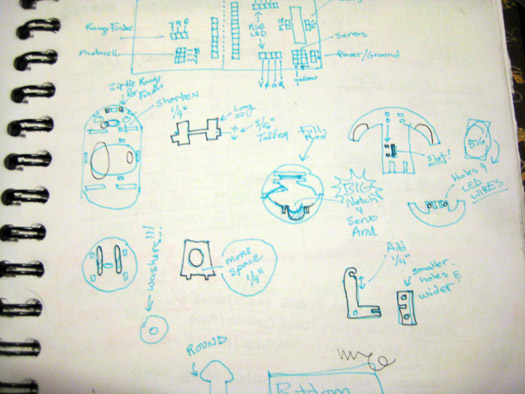
\includegraphics[width=3.5in]{img/memote-1-small.jpg} 
   \caption{Sketches for a robot built mostly with laser-cut parts.}
   \label{fig:memote-sketches}
\end{figure}

Figure \ref{fig:memote-sketches} shows a page from a designer's
sketchbook. These drawings were made in the middle of a design process
that had already involved physical prototypes. They were made to think
about details of robot parts before moving to Adobe Illustrator to
create a cutfile. SkruiFab will allow designers to make these kinds of
rough drawings without interruption or distraction.

There are a number of distinct drawings on the page. An ink fragment
may be part of a stencil boundary, or an arrow (or indicator line), or
words, or numeric dimensions. SkruiFab will enable designers to begin
with freeform drawings like these and use them as the basis for making
a structured cutfile iteratively.

SkruiFab will understand most of the sketch input shown in this
sketchbook. It doesn't need to make sense of everything, however. Ink
such as the pointy boundary surrounding the words ``BIG Notch'' does
not need to be understood. It \textit{does}, however, need to be
possible to tell the system that such ink can be ignored.

The system will understand the following input:

\begin{packed_enum}
\item Stencil boundaries
  \begin{packed_enum}
  \item Can represent outside edges or internal edges (holes)
  \item Boundaries can be lines or curves
  \end{packed_enum}
\item Arrows that relate one element to another
\item Text and numbers (descriptive names or parameter)
\item Dimension values (lengths and angles)
\item Guides
  \begin{packed_enum}
  \item Guide lines (dashed or dotted lines)
  \item Circuilar guides (dashed or dotted lines)
  \item Reference points (made by drawing thick dots)
  \end{packed_enum}
\item Hatching to indicate something different about a region
\item Erasure marks to remove/ignore something
\item Overtrace to existing ink to edit it
\item Graphic parameters
  \begin{packed_enum}
  \item Square bracket to indicate 90-degree angles
  \item Circular arc inside angle to vaguely indicate angle
  \item Tick marks on similar length to indicate same length
  \end{packed_enum}
\item Camera gestures
  \begin{packed_enum}
  \item Zoom in or out (continuous circular gesture)
  \item Pan on 2D plane (widget after zoom gesture, perhaps make a pan gesture)
  \end{packed_enum}
\end{packed_enum}

\end{document}  
